% `template.tex', a bare-bones example employing the AIAA class.
%
% For a more advanced example that makes use of several third-party
% LaTeX packages, see `advanced_example.tex', but please read the
% Known Problems section of the users manual first.
%
% Typical processing for PostScript (PS) output:
%
%  latex template
%  latex template   (repeat as needed to resolve references)
%
%  xdvi template    (onscreen draft display)
%  dvips template   (postscript)
%  gv template.ps   (onscreen display)
%  lpr template.ps  (hardcopy)
%
% With the above, only Encapsulated PostScript (EPS) images can be used.
%
% Typical processing for Portable Document Format (PDF) output:
%
%  pdflatex template
%  pdflatex template      (repeat as needed to resolve references)
%
%  acroread template.pdf  (onscreen display)
%
% If you have EPS figures, you will need to use the epstopdf script
% to convert them to PDF because PDF is a limmited subset of EPS.
% pdflatex accepts a variety of other image formats such as JPG, TIF,
% PNG, and so forth -- check the documentation for your version.
%
% If you do *not* specify suffixes when using the graphicx package's
% \includegraphics command, latex and pdflatex will automatically select
% the appropriate figure format from those available.  This allows you
% to produce PS and PDF output from the same LaTeX source file.
%
% To generate a large format (e.g., 11"x17") PostScript copy for editing
% purposes, use
%
%  dvips -x 1467 -O -0.65in,0.85in -t tabloid template
%
% For further details and support, read the Users Manual, aiaa.pdf.


% Try to reduce the number of latex support calls from people who
% don't read the included documentation.
%
\typeout{}\typeout{If latex fails to find aiaa-tc, read the README file!}
%


\documentclass[]{aiaa-tc}% insert '[draft]' option to show overfull boxes

 \usepackage{varioref}%  smart page, figure, table, and equation referencing
 \usepackage{wrapfig}%   wrap figures/tables in text (i.e., Di Vinci style)
 \usepackage{threeparttable}% tables with footnotes
 \usepackage{dcolumn}%   decimal-aligned tabular math columns
  \newcolumntype{d}{D{.}{.}{-1}}
 \usepackage{nomencl}%   nomenclature generation via makeindex
  \makeglossary%
 % \usepackage{subfigure}% subcaptions for subfigures
 % \usepackage{subfigmat}% matrices of similar subfigures, aka small mulitples
 \usepackage{subcaption}
 \usepackage{fancyvrb}%  extended verbatim environments
  \fvset{fontsize=\footnotesize,xleftmargin=2em}
 \usepackage{lettrine}%  dropped capital letter at beginning of paragraph
 \usepackage[colorlinks]{hyperref}%  hyperlinks [must be loaded after dropping]
 \usepackage{setspace}
 \doublespacing

 \title{Passive Haptics to Enhance Virtual Reality Simulations}

 \author{Richard Joyce\thanks{Ph. D. Candidate, Mechanical and Aerospace Engineering, Student Member AIAA.}
  \ and Stephen K. Robinson\thanks{Director – UC Davis Center for Human/Robotics/Vehicle Integration and Performance, Professor – Mechanical and Aerospace Engineering, Member AIAA.}\\
  {\normalsize\itshape University of California, Davis, Davis, CA 95616}\\
 }

 % Data used by 'handcarry' option if invoked
 \AIAApapernumber{YEAR-NUMBER}
 \AIAAconference{Modeling and Simulation Technologies Conference, January 2017, Dallas, TX}
 \AIAAcopyright{\AIAAcopyrightD{YEAR}}

 % Define commands to assure consistent treatment throughout document
 \newcommand{\eqnref}[1]{(\ref{#1})}
 \newcommand{\class}[1]{\texttt{#1}}
 \newcommand{\package}[1]{\texttt{#1}}
 \newcommand{\file}[1]{\texttt{#1}}
 \newcommand{\BibTeX}{\textsc{Bib}\TeX}

\begin{document}

\maketitle

\begin{abstract}
Recent advances in virtual reality technology have renewed interest in the use of head-mounted display based aerospace simulation.
We present work on a virtual reality system that combines low fidelity physical prototypes, providing what is commonly called ``passive haptics'', with high fidelity visuals provided by a virtual reality head-mounted display.
Interaction with the prototype is achieved using an optical hand tracker.
We evaluate the system with a Fitts' ISO9241-9 experiment on a virtual panel with 20 subjects.
Fitts' throughput was significantly increased with the passive haptics, and training time was decreased.
Subjective feedback from the subjects indicate they prefer the passive haptics for interacting with the virtual panel, and feel they are performing faster and more accurately.
The use of this type of simulator has applications in prototyping cockpit designs, as well as for training in deployed situations where resources are minimal.
\end{abstract}

\section{Introduction}
\lettrine[nindent=0pt]{T}{he} motivation for the prototype and experimental study described in this paper stems from the design of complex human-machine interfaces, particularly cockpits for spacecraft and high performance aircraft.
A common problem is that the design (or modernization) of a cockpit will go into flight before evaluation pilots are completely satisfied with the design process, due to time and budget concerns.
The remaining deficiencies of the cockpit design are expected to be overcome through additional crew training.
These deficiencies represent a cost throughout the lifetime of the vehicle in training, and ``unknown'' deficiencies of the human-machine system are often discovered too late in accident reports.
To address these issues, we have designed and prototyped a system to allow evaluations to occur earlier and more frequently in the design process.
The aim of our system is to give a non-functioning geometric mockup the interactivity of a simulator.
The mockup, which is used in the early stage of the design process, can now be used for more extensive cockpit evaluations, with a quicker iteration time than a simulator requires.
Our prototype, named the ``Rapidly Reconfigurable Research Cockpit'', consists of a virtual reality (VR) headset, optical hand tracking device, and 3D printed cockpit surfaces (Figure~\ref{fig:r3c})\cite{joyce_rapidly_2015}.

\begin{figure}[tb]
  \centering
  \begin{subfigure}{.49\textwidth}
    \centering
    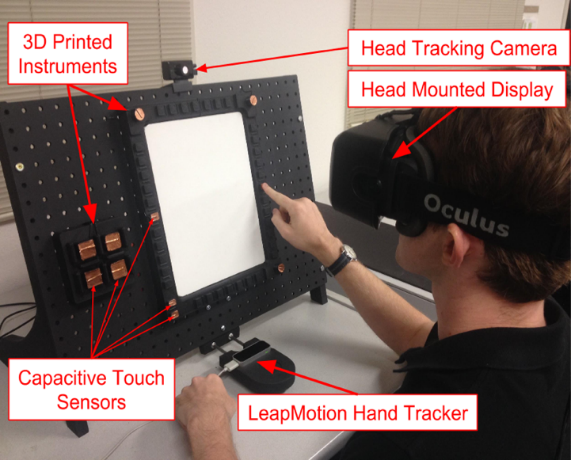
\includegraphics[width=.99\linewidth]{figures/r3c_callout.png}
    \caption{Subject using the system with major components annotated.}
    \label{fig:r3c_sub1}
  \end{subfigure}
  \begin{subfigure}{.49\textwidth}
    \centering
    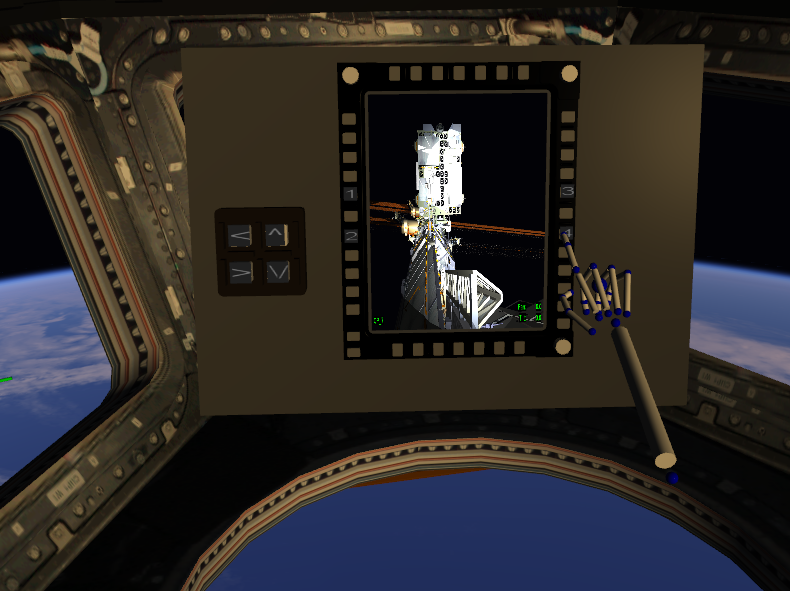
\includegraphics[width=.99\linewidth]{figures/virtual_world.png}
    \caption{View presented to the user in the virtual world.}
    \label{fig:r3c_sub2}
  \end{subfigure}
  \caption{Rapidly Reconfigurable Research Cockpit}
  \label{fig:r3c}
\end{figure}

The VR head-mounted display (HMD) provides a virtual view of the cockpit environment.
A challenging aspect of immersive VR simulations like this, however, is to provide appropriate tactile feel of the objects being interacted with (in this case, the instruments of a cockpit).
We solve this by using 3D-printed instruments co-located with the virtual environment, which is a technique commonly called ``passive haptics''.
The instruments remain inert and non-functioning in the real world, but appear fully functional in the virtual world presented to the user.
The user can interact with the virtual cockpit (i.e.\ pressing buttons) with the use of the optical based hand tracker, which measures the position of the users hands.
This position is used to determine if the user is activating a button.
Measurements from the hand tracker are used to display the essential visual feedback of hand position in the virtual world, as the use of an HMD blocks the view of ones own limbs.

We evaluate our prototype using a Fitts' Law task to quantify the effect of having passive haptics to a traditional virtual reality HMD simulation, which would provide no haptic feedback.
An experimental study with 20 subjects was performed and results are presented.
In addition to Fitts' Law performance, we also measured subjects reported fatigue and presence.

\section{Background}
\subsection{Fitts' Law}
One of the most well studied relationships for human-computer input is Fitts' Law\cite{fitts_information_1954}.
Fitts' Law states that the movement time of human targeting motion is related to the size of the target (W) and the distance to the target (D).
These two geometrical parameters are combined in the index of difficulty (ID), which is presented here in the popular Shannons' Formulation\cite{mackenzie_note_1989}:
\begin{equation}
  ID=\log_2\left(\frac{D}{W}+1\right)
  \label{eq:id}
\end{equation}
The index of difficulty is linearly proportional to the movement time (MT), which provides the Fitts' Law relationship:
\begin{equation}
  MT=a+b \cdot ID
\end{equation}
When comparing experimental conditions, it is recommended to use the measure of throughput (TP)\cite{soukoreff_towards_2004}.
This provides a single measure that encompasses speed and accuracy, averaging over the range of indices of difficulty.
Throughput has the units of bits per second, analogous to the amount of information, and is defined as the index of difficulty over the movement time:
\begin{equation}
  TP=\frac{ID}{MT}
  \label{eq:tp}
\end{equation}
In studies of Fitts Law in which subjects are performing the task in two dimensions the ISO9421-9 circle multi-directional tapping task has become the standard\cite{international_organization_for_standardization_iso_2000}.
A diagram of the circle task is shown in Figure~\ref{fig:circle}.
An important consideration of Fitts' Law experiments is to utilize the adjustment for accuracy.
This uses the recorded endpoint data to adjust for how the subjects actually performed the task.
For example, often subjects will only use a smaller portion of a large target, meaning the width they performed is smaller than the width presented.
The effective target width, $W_e$, is used to account for this, and is defined as the width which encompasses 96\% of the endpoints, assuming a normal distribution of endpoints.
This can be calculated by the standard deviation of endpoint positions along the direction of movement ($\sigma$), where $W_e = 4.133\sigma$.
The effective width can then be used in Equation~\ref{eq:id} instead of the presented width, $W$.

\begin{figure}[htb]
  \centering
  
\includegraphics[width=0.45\textwidth]{figures/iso9241.png}
  \caption{ISO9241 Fitts' Circle or multi-directional tapping task. D = distance, W = width.}
  \label{fig:circle}
\end{figure}

There have been numerous studies evaluating Fitts' Law in novel virtual environments and novel input devices.
Chun et al.\cite{chun_evaluating_2004} evaluated a set of 3D stereo displays with a single haptic-enabled stylus using a Fitts tapping task.
Teather \& Stuerzlinger\cite{teather_pointing_2011} performed a fully 3D targeting task using a hand tracker.
Liu et al.\cite{liu_comparing_2009} performed a planar multi-directional Fitts' task with a stereoscopic display, and compared virtual world to real world results, finding movement time twice as long in the virtual condition.
Kohli et al.\cite{kohli_redirected_2012} evaluated passive haptics with warped virtual space to fool the user of the nature of the physical world.
They had the subjects perform an ISO9241-9 Fitts' circle on a panel placed in front of them, and in some conditions the panel was rotated in the virtual world but not in the real world to create the discrepancy.
The subjects hand movement was warped to compensate for this.
Seixas et al.\cite{seixas_one_2015} performed an ISO 9241-9 Fitts' circle task with the same LeapMotion hand tracker we use, but did not employ any haptic feedback.
Our study is a unique combination of using a head-mounted display, passive haptics and non-obtrusive hand tracker.

\subsection{Passive Haptics}
A constant challenge of virtual environments has been presenting the user with a tactile sensory input that matches the visual sensory inputs they are experiencing.
One focus of this work is the idea of passive haptics, whereby we recreate the tactile environment to provide the sense of touch and external forces.
The disadvantage is that the tactile environment cannot dynamically change during the simulation.
Fortunately, the adaptability (during simulation) of the passive haptic environment is not a requirement for the use case of aerospace cockpit simulation.
We still retain the ability to quickly change the environment via 3D printing new parts in between simulation sessions.

Previous work of passive haptics has shown promising results for increased presence or task performance.
Schiefele et al.\cite{schiefele_simple_1998} used a head-mounted display (HMD) to replace the visuals of a flight simulator (though technology has drastically changed in HMDs and hand tracking since their publication).
They recreated only the positions of the panels with a flat plate and then used a magnetic hand tracker for reading the pilot input.
A short usability study was presented, and they found that users could activate switches, knobs and dials in less time with the physical panel than without (i.e.\ reaching into mid-air), a result reproduced here.
Insko\cite{insko_passive_2001} investigated the impact of passive haptics on generic virtual environments.
It was found that the passive haptics increased the sense of presence felt by users.
An experiment had two groups complete a maze in a virtual environment, one group with passive haptics on boundaries, and one without.
After training the passive haptic group bumped into far fewer obstacles than the group without.
Borst and Volz\cite{borst_evaluation_2005} created a ``mixed'' haptic virtual environment, whereby they combined an active haptic glove with a passive haptic panel.
They found the glove by itself consistently performed worse than the other two, but overall no significant difference existed between passive haptics and their mixed haptics, again indicating the power of simple passive haptics.

\section{Methods}
\subsection{Technical Details}
The head mounted display used is an Oculus Rift Development Kit 2.
The hand tracker, LeapMotion, is mounted above and pointed down so the field of view encompasses the area in front of the panel.
A custom calibration program is run to line up the LeapMotion measurements with the virtual world in the rendering engine.
For the experiment reported here, a blank panel (45cm x 45cm) was used to provide only the backstop of the virtual buttons for the ``Passive Haptics'' condition.
Subjects were seated in front of the panel.
The button selection is registered by the subject moving their index finger into a hover zone (cylinder for the circle buttons used) in front of the button that extends outward 2.54cm and inward 1.27cm.
Their entrance into the hover zone is indicated to them by the button changing color.
A successful button press is registered after staying in the hover zone for 160ms, and is indicated by the color turning off and a button click noise being played over speakers.

The authors previous study asked subjects to complete a discrete button targeting task, and validated our technical approach\cite{joyce_rapidly_2015}.
Subjects were able to select the buttons in the virtual world as accurately as in the real world, albeit with a small time penalty, consistent with other studies comparing real world to virtual world inputs\cite{liu_comparing_2009}.
However, the difference between the passive haptic and no passive haptic condition was insignificant, leading to a more extensive Fitts' evaluation that is presented in this paper.
The experimental setup for this study consisted of two conditions, one with the panel (``Passive Haptics (PH)'') and one without the panel (``No Passive Haptics (NH)''), where the subjects would need to target the buttons in mid-air.
The different conditions and the view of the virtual world is shown in Figure 3.

\begin{figure}[tb]
  \centering
  \begin{subfigure}{.32\textwidth}
    \centering
    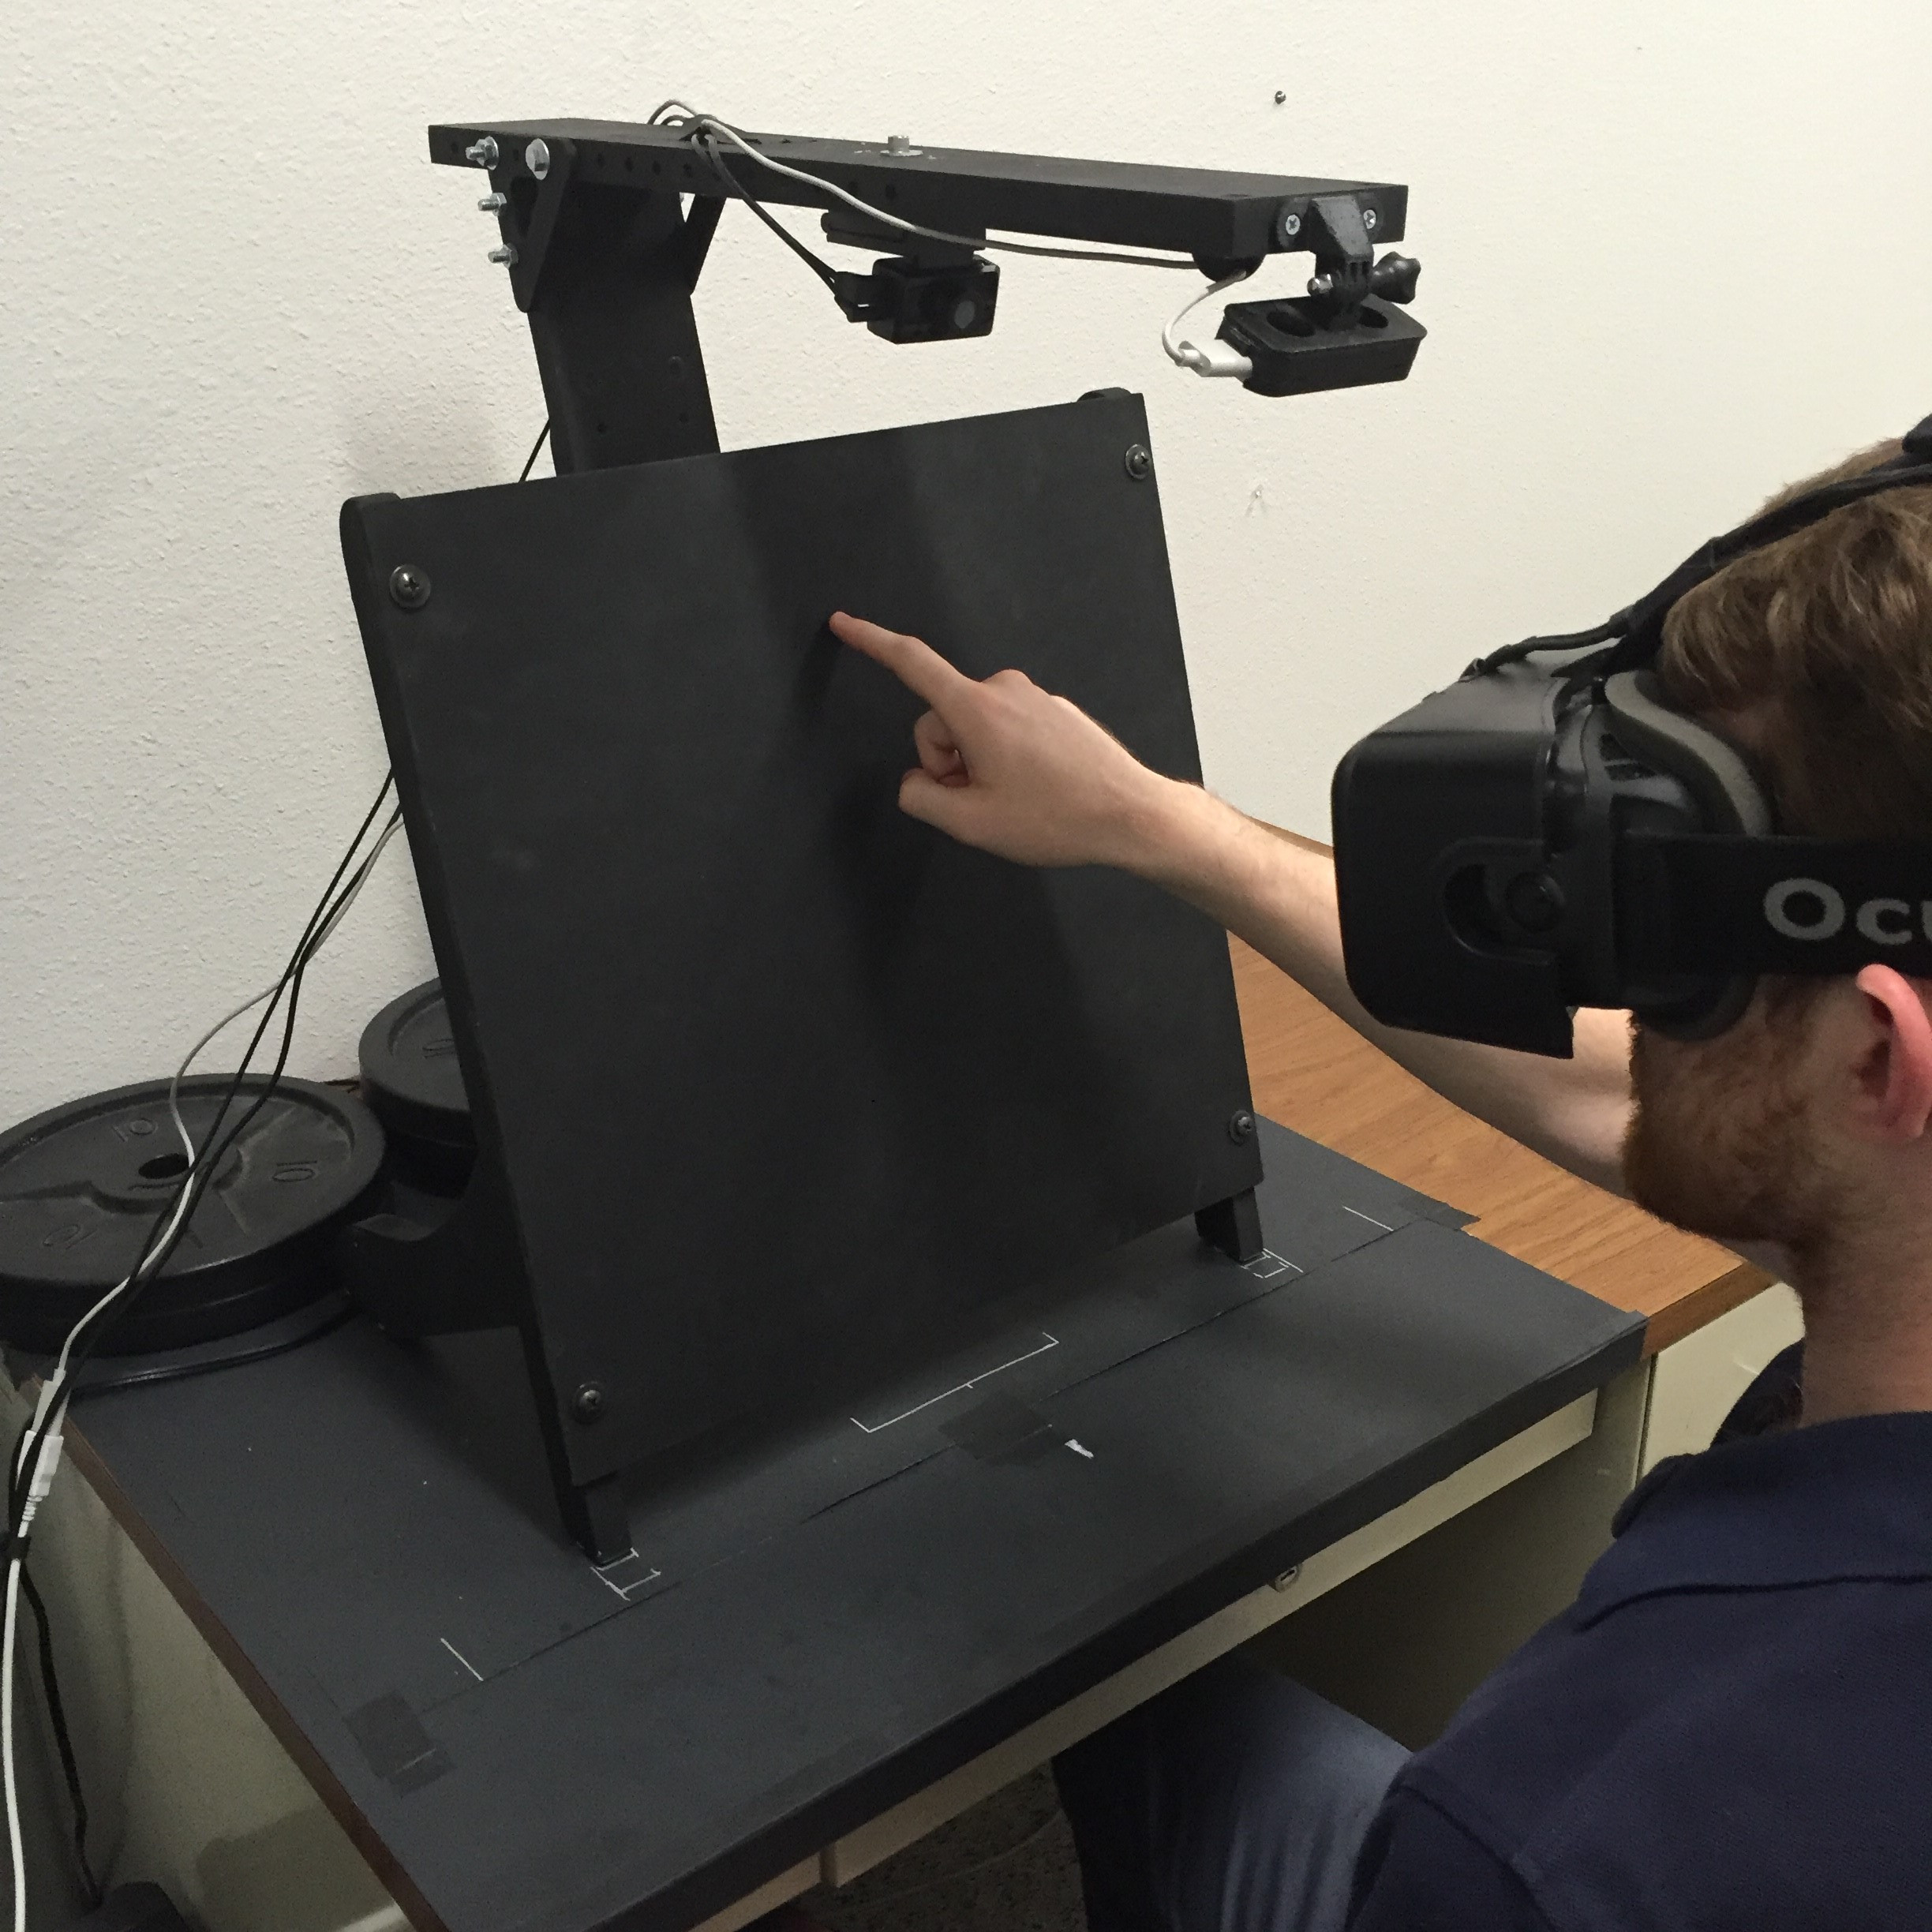
\includegraphics[width=.99\linewidth]{figures/passive_haptics.jpg}
    \caption{\textit{Passive Haptics} condition}
    \label{fig:passive_haptics}
  \end{subfigure}
  \begin{subfigure}{.32\textwidth}
    \centering
    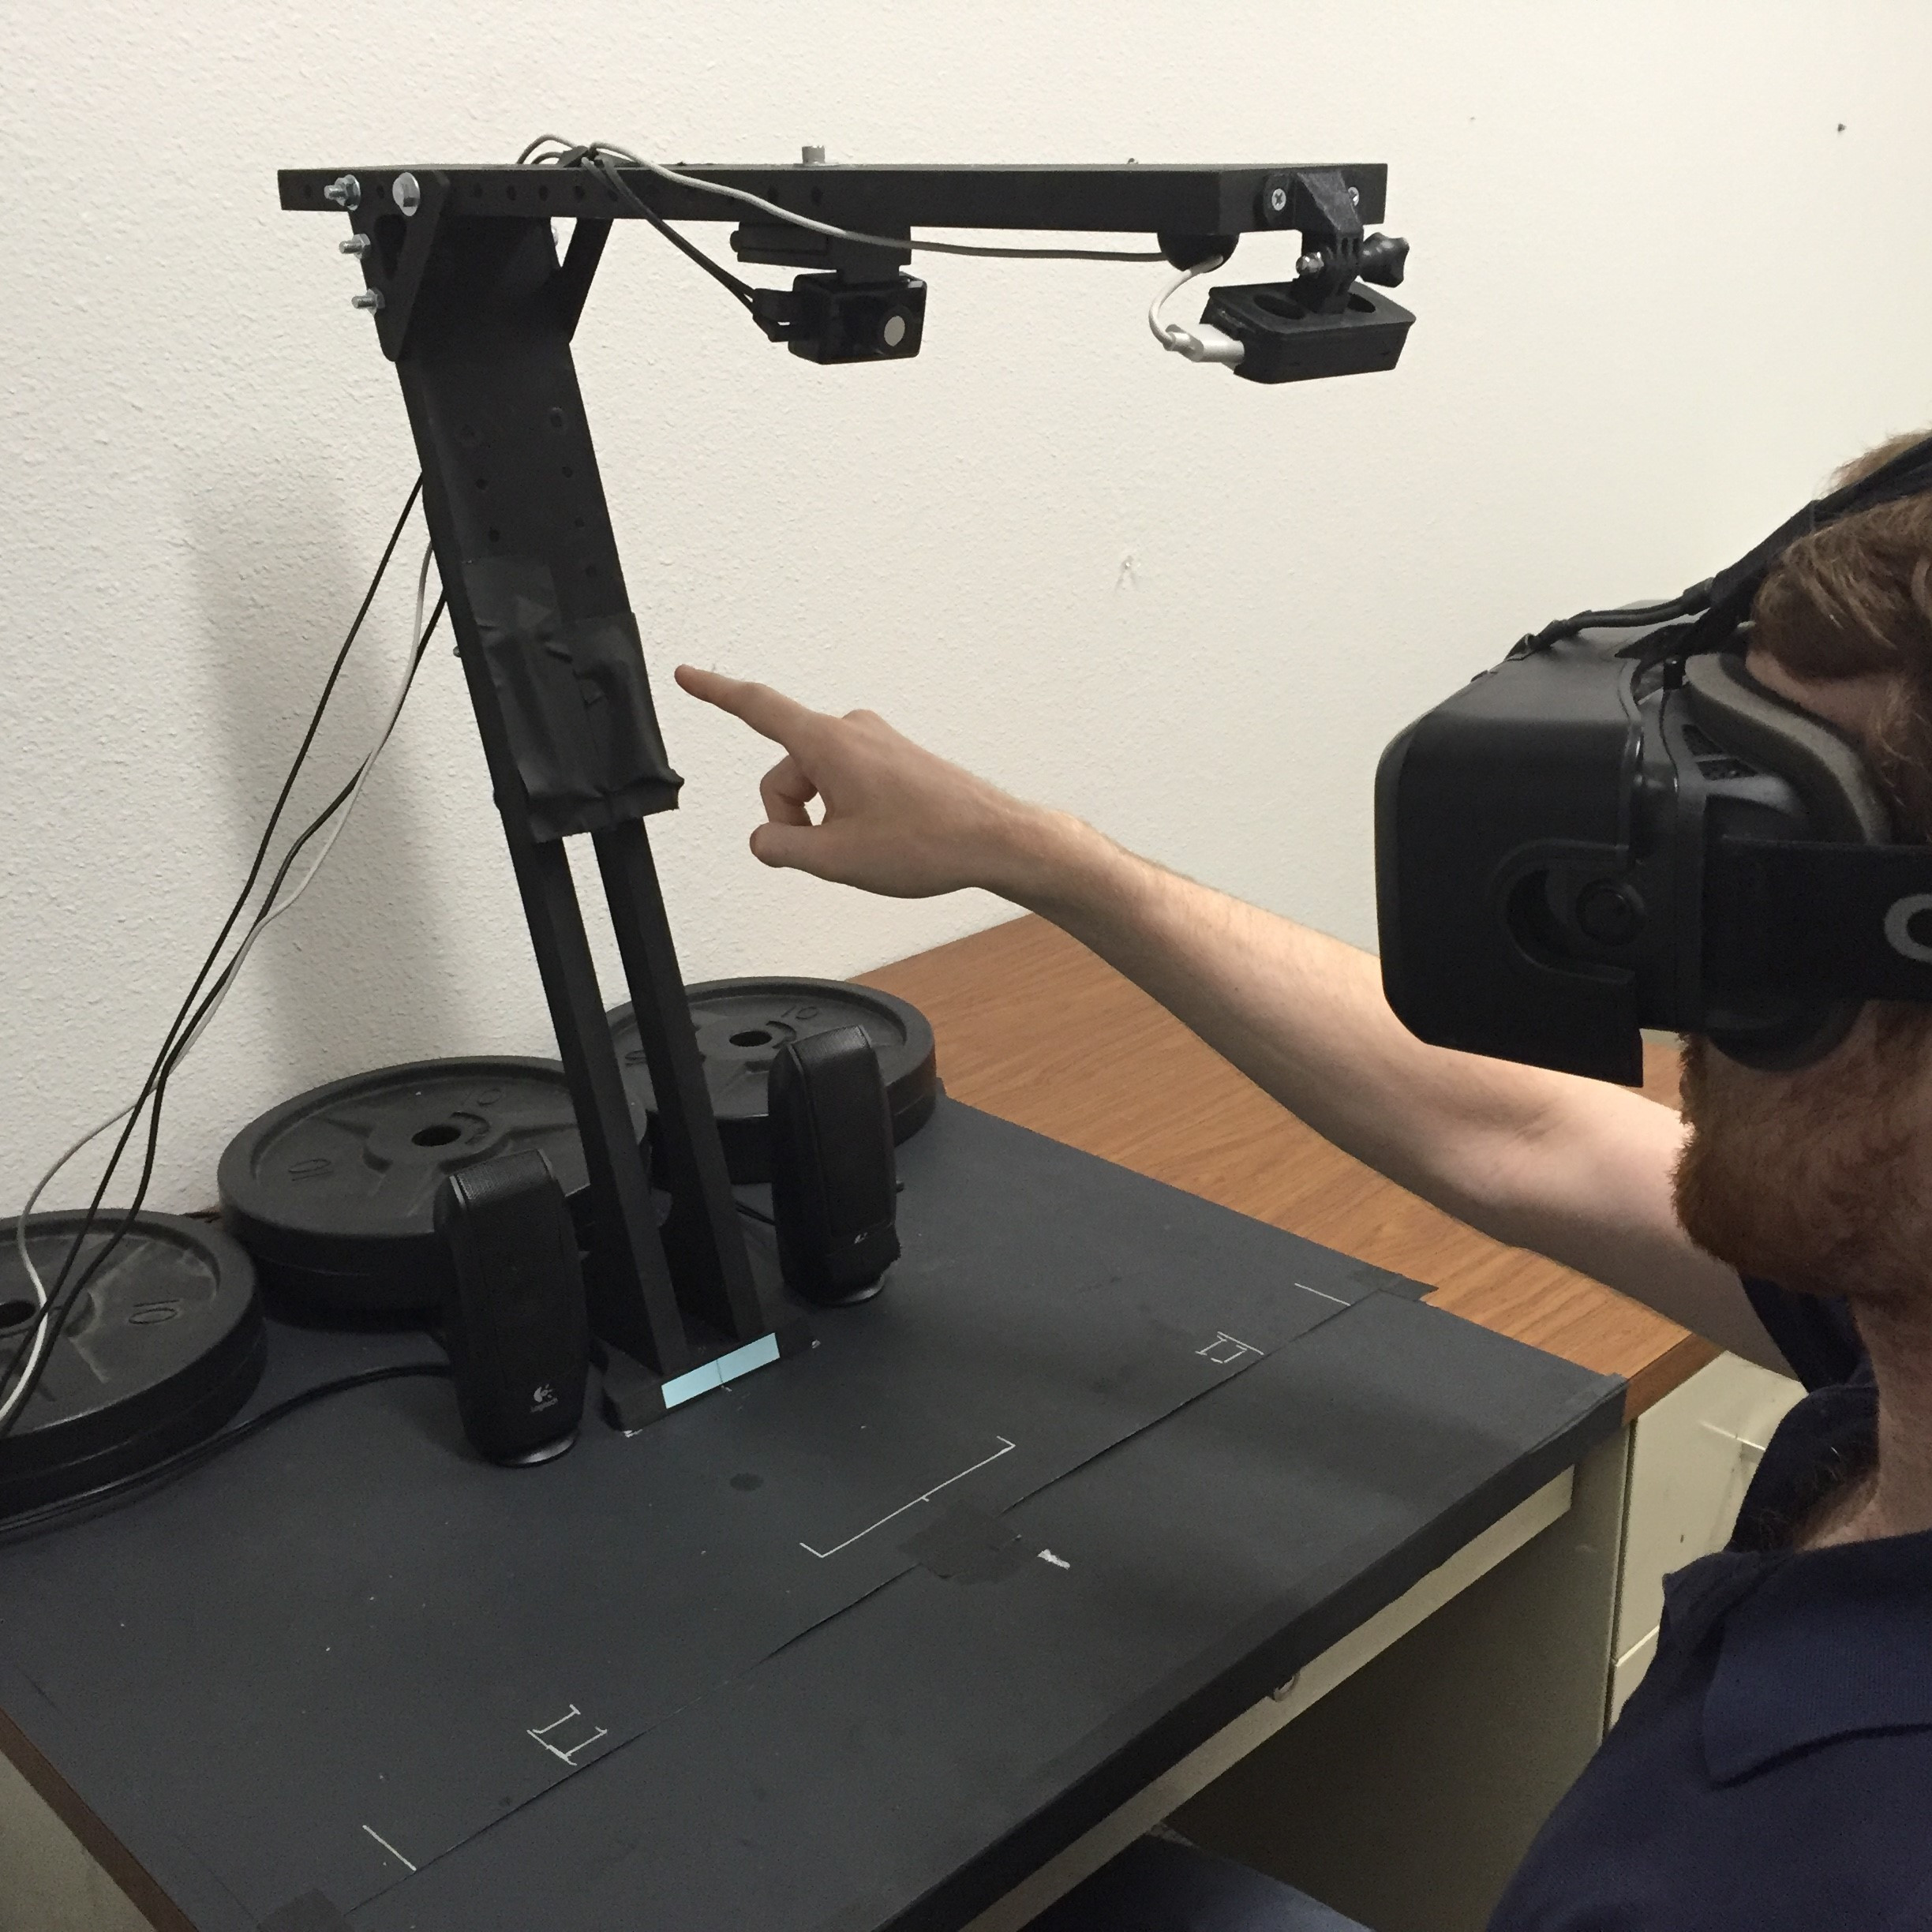
\includegraphics[width=.99\linewidth]{figures/no_passive_haptics.jpg}
    \caption{\textit{No Passive Haptics} condition}
    \label{fig:no_passive_haptics}
  \end{subfigure}
  \begin{subfigure}{.32\textwidth}
    \centering
    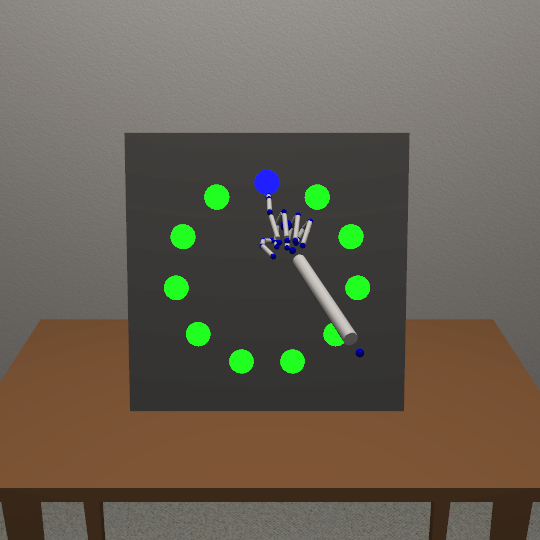
\includegraphics[width=.99\linewidth]{figures/virtual_view.png}
    \caption{Virtual world view}
    \label{fig:virtual_view}
  \end{subfigure}
  \caption{Experimental Setup}
\end{figure}

\subsection{Experimental Task}
Subjects were asked to complete 15 configurations of the Fitts' ISO9241-9 circle, as shown in Figure~\ref{fig:circle}.
The configurations were comprised of 3 distances (D) of 20cm, 30cm and 40cm and 5 widths (W) ranging from 5mm to 25mm in 5mm increments.
Every circle contained 11 targets.
They performed each circle sequence three times in a row before proceeding to the next configuration.
The target width order was chosen randomly, but the order of the distances was sequenced from smallest to largest for half of the subjects, and largest to smallest for the other half.

The 15 circle configurations were completed for each subject in both conditions, with passive haptics and with no passive haptics.
The order of the conditions was counterbalanced so that half saw the passive haptic condition first.
Subjects were not instructed on the second condition before they finished the first condition (i.e.\ subjects who started with no passive haptics were not told the second half would proceed with a passive haptic in place, and could not see the real panel in the experimental room).
At the conclusion of each condition, they were given a presence questionnaire of 21 questions on a 7 point Likert scale, with questions from the Presence Questionnaire and Slater-Usoh-Steed questionnaire.
At the conclusion of the experiment, a condition comparison questionnaire was administered to directly compare subjects perceptions of the two conditions, with a 7 point Likert scale anchored from ``With Panel'' to ``Without Panel''.
The subjects were asked after every other circle completion to provide an arm fatigue rating based on the Borg RPE (Rating of Perceived Exertion) scale (between 6-20).

\section{Results \& Discussion}
Twenty (20) subjects performed the experiment, all engineering students (undergraduate and graduate).
Their ages ranged from 19-30, and included 10 female and 10 male subjects (balanced between the groups).
All subjects had less than an hour experience with virtual reality devices, with half indicating no previous experience.
Subjects used their dominant hand index finger to target the buttons (two subjects were left-handed).

\subsection{Data Reduction}
Typical Fitts' Law studies only use measurements after the subject is well trained in the task.
This is usually quantified by the throughput (Equation~\ref{eq:tp}) increasing until it reaches an asymptote.
Since we wanted to investigate the learning effects we did not require the subjects to reach this asymptotic behavior, expecting subjects to learn the system quickly (and observing so much during the data collection).
Instead, we filtered the movements afterward to select only those which were direct to the target.
There were 18,000 movements recorded total (20 subjects, 2 conditions, 15 circle configurations with 30 movements each).
This section briefly describes the methods to reduce the movements to only the ones in which the subject moved direct to the target.

Human targeting motions are known to consist of a ballistic and a corrective phase\cite{woodworth_accuracy_1899}.
We consider a single target-to-target movement for the Fitts' Law analysis if it is predominantly ballistic, and the ballistic portion covers the majority of the distance to the target.
Mathematically, the ballistic portion is determined by finding the maximum velocity and the corresponding minimums on either side.
This can be seen in plots of the movements in Figure~\ref{fig:movements}.
The movement was considered predominantly ballistic if time spent in the ballistic phase is more than 85\% of total time, and the ballistic phase path distance was at least 75\% of the distance between the targets.
We also removed movements which had a total path distance more than 125\% of the distance between the targets, or travelled more than 1.3in after entering and exiting the target (but not successfully activating it).
This left 12,300 movements categorized as ``good movements'' for the Fitts analysis.

\begin{figure}[p]
  \centering
  \begin{subfigure}{.49\textwidth}
    \centering
    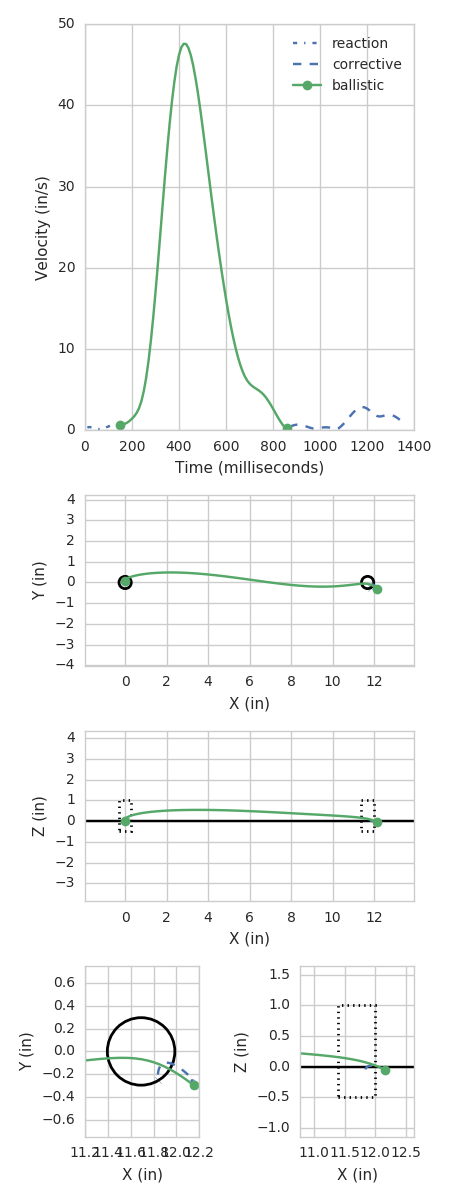
\includegraphics[width=.99\linewidth]{figures/mvmt6467.png}
    \caption{Passive Haptics condition, D=30cm, W=15mm.}
    \label{fig:mvmt_sub1}
  \end{subfigure}
  \begin{subfigure}{.49\textwidth}
    \centering
    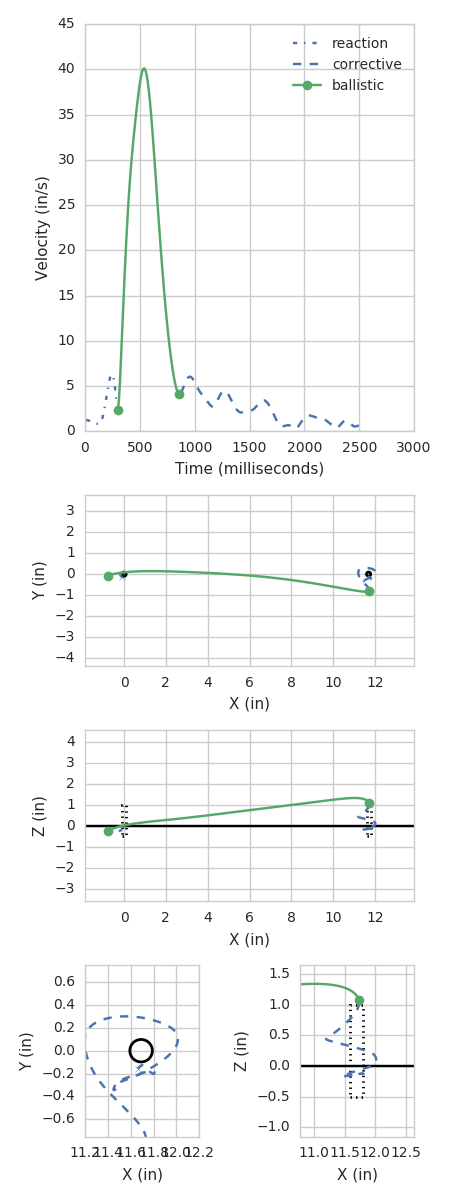
\includegraphics[width=.99\linewidth]{figures/mvmt3831.png}
    \caption{No Passive Haptics condition, D=30cm, W=5mm.}
    \label{fig:mvmt_sub2}
  \end{subfigure}
  \caption{Example trajectories of single target movements. Velocity profile on top, with XY and XZ position views shown underneath, followed by closeup views of the target finish. Starting target is at (0,0).}
  \label{fig:movements}
\end{figure}

In order to ensure the subject had reached familiarity for a particular block (a single distance and width configuration consisting of 30 movements), we only considered blocks with 20 or more good movements.
After removing movements from poorly performed blocks, the movement count was 9,107, just over half of the original movements.
Of these, 5,612 were from the passive haptics conditions, while only 3,495 were from the no haptics condition.
This speaks to the extra difficulty subjects had in learning the no haptics condition, a common theme of our results.
The removal of poorly performed blocks was also required for a proper adjustment for accuracy, as this calculation must be performed per subject per block.
The endpoint position recorded by the hand tracker was used for the adjustment for accuracy.

\subsection{Fitts' Law}

The regression plot is shown in Figure~\ref{fig:fitts}, and the parameters are listed in Table~\ref{tab:fitts}, along with the throughput calculation.
The throughput of each condition is calculated as a mean-of-means, whereby first a mean for each index of difficulty for each subject is found, before averaging between subjects.
The regression and throughput used the effective index of difficulty for their calculation.
Movement time started when the previous target was activated (providing a visual and audible feedback), and ended either when the goal target was activated, or when the subject stopped moving (less than 5\% of peak velocity) within the target zone, whichever came first.
This adjustment accounted for a maximum discrepancy of 160ms, the time required to stay in the target zone.

The slope of the two conditions were almost identical, but the no haptics condition had a higher intercept.
The difference in throughput was 0.6 bps, with passive haptics providing a higher throughput at 4.7bps.
The throughput for both is similar to the range of throughput found in literature for a computer mouse (3.7-4.9bps)\cite{soukoreff_towards_2004}, but low for direct manipulation devices (6.5bps)\cite{mackenzie_fitts_2015}.

Our passive haptics condition is a similar setup to one condition tested in Kohli et al.\cite{kohli_redirected_2012}.
They used a marked fingertip tracker instead of our marker-less approach, but had subjects perform a Fitts circle on a physical panel while wearing an HMD.
They found a throughput value of \~6bps for this condition, compared to our result of 4.7bps.
It is possible that the performance of their hand tracker contributed to a higher throughput.
Seixas et al.\cite{seixas_one_2015} performed a similar condition to our NH condition, using a LeapMotion to perform a Fitts circle, though visual feedback was given on a computer monitor.
Their results found a throughput of \~2.9bps, much lower than our value of 4.1bps.
This performance improvement in our experiment is likely due to the additional immersion of having a head-mounted display.

\begin{figure}[htb]
  \centering
  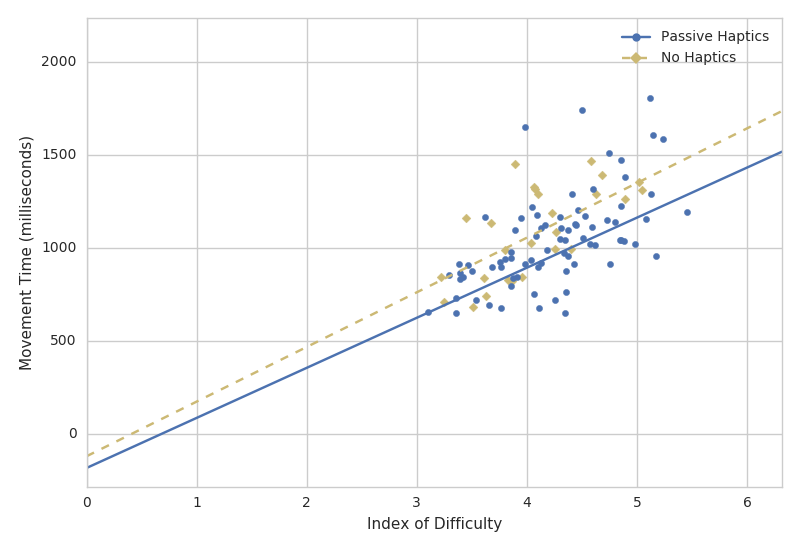
\includegraphics{figures/fitts.png}
  \caption{Fitts' Law regression. Points are mean of each circle configuration for each subject. Regression parameters shown in Table~\ref{tab:fitts}}
  \label{fig:fitts}
\end{figure}

\begin{table}
  \centering
  \begin{tabular}{lccc}
    Condition &  Throughput (bps) &  Slope (msec/bit) &  Intercept (msec) \\
    \hline\hline
    No Haptics  &          4.1 &        294 &       -117 \\
    Passive Haptics &          4.7 &        269 &       -180 \\
  \end{tabular}
  \caption{Fitts' Law analysis results.}
  \label{tab:fitts}
\end{table}

\subsection{Subjective Results}

The presence questionnaires given after each condition were scored by summing the response for each question (from 1-7) for each subject to create their ``Presence Score'' and the mean for each condition is presented in Table~\ref{tab:subjective}.
We separate the groups by which condition they performed first.
The only significant change is for the subjects who lose the physical panel for their second condition score a lower presence rating.
This is interesting as the subjects who lost the panel performed the same (measured by throughput) in the second NH condition as those who started with the NH condition, so only the presence score indicates a difference between these two datasets.
The loss of presence score for subjects who lost the panel indicates that they found the panel more immersive, yet the subjects who gained the panel either did not find it added significantly to their experience or they had already maxed out their ratings on the Likert-scale.
The answers to the final question of the condition comparison shown below refutes the former as most subjects strongly preferred the panel.

The average arm fatigue score reported at the end of the first condition was significantly higher for those whose first condition was NH compared to those starting with PH.
This result is also reported in Table~\cite{tab:subjective}.
The underlying cause of this could be the aid of passive haptics in performing the task (as seen with the higher throughput), causing less time to be spent moving the arm, or it could also be a biomechanical cause.
One biomechanical reason could be due to subjects being able to hit the panel with non-zero velocity to activate the button in the PH condition, yet they had to achieve zero velocity on their own without the panel in the NH condition.
The final score after the second condition was not significantly different, which is possibly due to subjects plateauing at their maximal fatigue for the experiment

\begin{table}
  \centering
  \begin{tabular}{llccc}
    Sequence & Condition & Presence Score & Arm Fatigue & Time to Complete Condition (min) \\
    \hline\hline
    No Haptics First & 1. NH & 72.9 (3.1) & 15.0 (0.9) & 15.1 (1.0) \\
    & 2. PH & 73.8 (3.2) & 15.2 (1.0) & 11.9 (1.3) \\
    \hline
    Passive Haptics First & 1. PH & 70.4 (2.3) & 11.7 (1.1) & 10.9 (0.7) \\
    & 2. NH & 63.9 (2.0) & 14.5 (0.9) & 13.2 (0.9) \\
  \end{tabular}
  \caption{Results from questionnaires and elapsed time for each condition. Standard error of the mean is reported in parentheses. Presence Score is the average summation for each subject. Arm Fatigue is mean of each subjects final score reported for the condition (Borg RPE scale between 6-20).}
  \label{tab:subjective}
\end{table}

The results of the comparison questionnaire given to subjects at the conclusion of the experiment is summarized in Figure~\ref{fig:comparison}.
All subjects indicated that they preferred the PH condition (except for two who answered no preference).
Similar results were found when asking the subjects if they felt they performed faster or more accurately in one condition or the other, with the vast majority indicating they felt faster and more accurate in the Passive Haptics condition.
Most subjects felt that they fatigued more or quicker in the No Haptics condition, but this was not as heavily weighted to one side of the scale as the other results.
Finally, a direct question on presence had most answering that they felt they were actually in the virtual room more in the passive haptics condition.

\begin{figure}[htb]
  \centering
  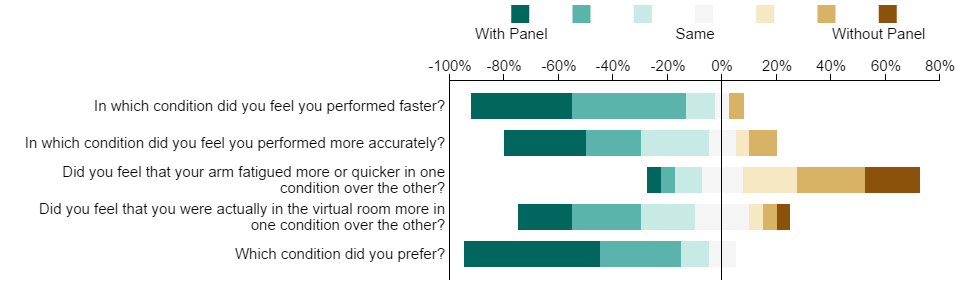
\includegraphics{figures/subjective.png}
  \caption{Results from condition comparison survey. Questionnaire given at end of experiments asking subjects to compare the two conditions. A 7-point Likert scale was used, anchored from ``With Panel'' to ``Without Panel''.}
  \label{fig:comparison}
\end{figure}

The average amount of time taken to complete the entire condition (15 circle configurations) for each subject is shown in Table~\ref{tab:subjective}, not including breaks between circles.
Overall, subjects were able to complete the passive haptics condition faster, but those who started with passive haptics were able to complete the no haptics condition almost 2 minutes faster (15.1 minutes to 13.2 minutes).
This implies a positive transfer of training for switching to no haptics after having passive haptics.
The reverse was observed for the other direction, with subjects performing the passive haptics condition slower by a minute after doing the no haptics condition.

The final result presented here is the average time spent in the corrective phase of the trajectory, grouped by condition and target distance, shown in Table~\ref{tab:corrective_time}.
In all cases, more time was taken for the corrective phase with No Haptics than in the Passive Haptics condition.
This is likely due to the passive haptics providing the correction for the Z-axis, allowing subjects to focus on correcting only two axes.

\begin{table}
  \centering
  \begin{tabular}{lccc}
    & \multicolumn{3}{c}{Corrective Time (msec)} \\
    Distance (cm) & 20 & 30 & 40 \\
    Condition & & & \\
    \hline\hline
    No Haptics &  533 (20) & 707 (21) & 1253 (40) \\
    Passive Haptics & 364 (15) & 500 (19) & 804 (35) \\
  \end{tabular}
  \caption{Average time spent in corrective movement per condition and target distance. Standard error of the mean in parentheses.}
  \label{tab:corrective_time}
\end{table}

\section{Conclusion}

We evaluated a hand-tracked, passive haptic interface for virtual reality head mounted displays using a Fitts ISO9241-9 multi-directional tapping task.
We found increased Fitts' throughput when subjects had a physical panel (passive haptics) in position with the virtual buttons than without a physical panel.
Subjects were able to train quicker in the virtual environment with the passive haptics than without.
Subjects perceived that they performed faster and more accurately with the passive haptics, and overall preferred the passive haptic condition.

% produces the bibliography section when processed by BibTeX
%\nocite{*}
\bibliography{MST2017}
\bibliographystyle{aiaa}

\end{document}

% - Release $Name:  $ -
